\documentclass[onecolumn,aps, pre,amsmath,amssymb,longbibliography,11pt]{revtex4-2}
\usepackage{graphicx}
% \usepackage{dcolumn}
\usepackage{bm}
\usepackage{amsfonts}
\usepackage{xcolor,tabu}
\usepackage{multirow}
\usepackage{amsthm}
\usepackage{textcomp}
\usepackage{tikz}
\usepackage[colorlinks=true,
            linkcolor=blue,
            urlcolor=blue,
            citecolor=blue]{hyperref}
\hypersetup{bookmarksopen=true}
\usepackage{xr}
\usepackage{float}



\begin{document}
\title{Does orientation of bacteria change the light attenuation?}

\author{Zhengyang Liu}
\date{\today}
\maketitle


In a previous note, we use a simple calculation to show that in the weak-attenuation limit, the orientation of an object does not affect the light attenuation.
In this note, we want to verify this hypothesis in experiment.

We take a video of a randomly reorienting bacterium in water.
If our hypothesis is valid, the light intensity, measured by the average pixel value, is a constant.
Due to the fact that the light source cannot be perfect and always has a fluctuation, our image cannot have a strictly constant light intensity.
We are not looking to obtain a constant light intensity in our experiment.
Instead, we estimate the fluctuation of the light source, and compare it with the fluctuation of the single bacterium image.

\begin{figure}[h]
  \begin{center}
    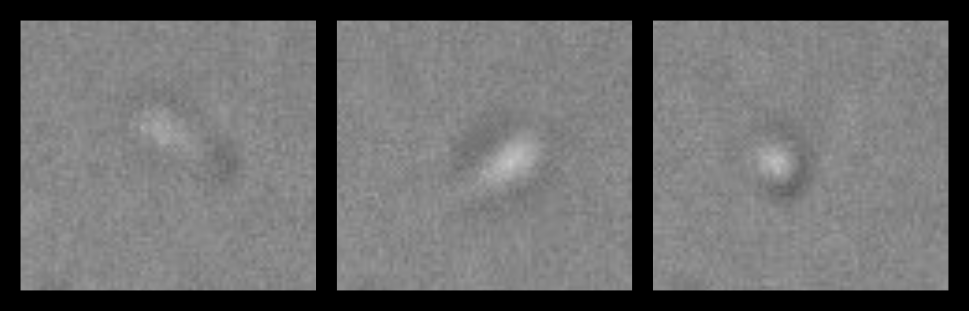
\includegraphics[width=5in]{orientation.png}
  \end{center}
  \caption[]{Three snapshots from a video of a single reorienting bacterium}
  \label{fig:orientation}
\end{figure}

Figure~\ref{fig:orientation} shows 3 snapshots of a single reorienting bacterium.
The total length of the video is 250 frames, shot at 30 frames per second.
This single bacterium video is cropped from a larger field of video, which contains several tens of bacteria.
Let's assume that the fluctuation of the larger field of view video is a good estimate of the fluctuation of the light source.
We will extract the intensity fluctuations of both the small video and the large video, and then compare them.
Figure~\ref{fig:results} shows the mean intensities of the one-bacterium video and the large field of view video over time.
Both intensities fluctuate, and the fluctuation of the one-bacterium video is much stronger.

\begin{figure}[h]
  \begin{center}
    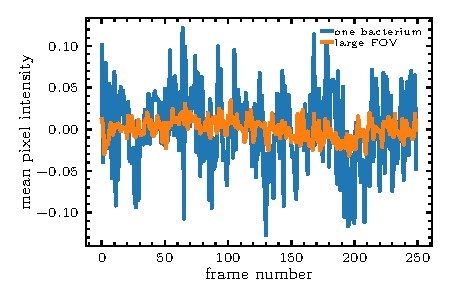
\includegraphics[width=5in]{orientation-results.pdf}
  \end{center}
  \caption[]{Mean intensities of the one-bacterium video and the large field of view video over time.}
  \label{fig:results}
\end{figure}

This result suggests that the orientation of bacteria may affect the local light attenuation.

\end{document}
